We have described an approach to parameterizing models of risk group dynamics
which hopefully highlights the
\textit{feasibility} of including such model components based on available data.
Next, we will explore the
\textit{importance} of including these components
through comparison of projected model outputs
across different implementations of risk group dynamics.
Specifically, we will first compare structural variants
involving differences in population growth, number of risk groups, and turnover.
Next, we will explore the impact of different rates of turnover on
overall and group-specific prevalence and incidence,
and on implications for model fitting.
% ==================================================================================================
\subsection{Model \& Simulations}\label{ss:model-sim}
We start with a simple deterministic SIR model of
transmission in a heterogeneous population,
which is meant to be representative of an arbitrary epidemic,
rather than any specific context or disease.
The model includes three health states:
susceptible~$\mathcal{S}$, infected~$\mathcal{I}$, and recovered~$\mathcal{R}$,
as shown in Figure~\ref{fig:health-states},
and $G = 3$ levels of risk:
high~$H$, medium~$M$, and low~$L$,
stratified by different rates of contact formation across groups.
Gender is not modelled.
Individuals in risk group $i$ are assumed to
form contacts at a rate $C_{i}$, and
the probability of contact formation between these individuals
with partners in risk group $\mathrm{i}$ is assumed to
be proportionate with the total number of available contacts:
\begin{equation}
  \rho_{\mathit{i}\mathrm{i}} = \frac
    {C_{\mathrm{i}} x_{\mathrm{i}}}
    {\sum_{\textsl{i}}C_{\textsl{i}} x_{\textsl{i}}}
\end{equation}
\begin{figure}
  \centering
  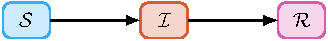
\includegraphics[width=0.4\linewidth]{health-states}
  \caption{Modelled health states}
  \label{fig:health-states}
\end{figure}
\par
Transmission of the infection from infected $\mathcal{I}$ to susceptible $\mathcal{S}$ individuals
is assumed to occur with probability $\beta$ per contact.
Recovered individuals $\mathcal{R}$ are not considered infectious,
but do not return to the susceptible state.
The force of infection for susceptible individuals in risk group $i$
is therefore modelled using the following equation:
\begin{equation}
  \lambda_{i} =
  C_{\mathit{i}}
  \sum_{\mathrm{i}}
  \rho_{\mathit{i}\mathrm{i}} \thinspace
  \beta \frac{\mathcal{I}_{\mathrm{i}}}{N_{\mathrm{i}}}
  \label{eq:foi}
\end{equation}
Infected individuals are assumed to be diagnosed and begin treatment at a rate $\tau$ (per year).
As described in Section \ref{s:system},
individuals enter the model at a rate $\nu$,
exit at a rate $\mu$,
and transition from risk group $i$ to group $j$ at a rate $\zeta_{ij}$.
The default parameters for this base model are summarized in Table~\ref{tab:params-base},
and the full system of model equations is given in \ref{aa:eqs-model}~\nameref{aa:eqs-model}.
\begin{table}
  \centering
  \caption{Base model parameters.
    All rates have units $\mathrm{year}^{-1}$ and durations are in $\mathrm{years}$.}
  \label{tab:params-base}
  \begin{tabular}{clc}
	\toprule
	    Symbol     & Description                                                             &                 Value                  \\
	\midrule
	 $\bm{\beta}$  & transmission probability per contact                                    &                 $0.03$                 \\
	    $\tau$     & rate of treatment initiation among infected                             &                 $0.1$                  \\
	    $N_0$      & initial population size                                                 &                 $1000$                 \\
	\midrule
	$\bm{\hat{x}}$ & proportion of system individuals: high, medium, low activity            & $[ 0.04 \enspace 0.20 \enspace 0.76 ]$ \\
	$\bm{\hat{e}}$ & proportion of entering individuals: high, medium, low activity          & $[ 0.04 \enspace 0.20 \enspace 0.76 ]$ \\
	$\bm{\delta}$  & average duration spent in: high, medium, and low activity groups        &    $[ 5 \enspace 15 \enspace 25 ]$     \\
	     $C$       & rate of contact formation among individuals: high, medium, low activity &     $[ 25 \enspace 5 \enspace 1 ]$     \\
	    $\nu$      & rate of population entry                                                &                 $0.05$                 \\
	    $\mu$      & rate of population exit                                                 &                 $0.03$                 \\
	\bottomrule
\end{tabular}
\end{table}
\par
Using this model (and variants, described below),
simulated epidemics are initialized at $t = 0$ with $N_0 = 1000$ individuals,
distributed according to $\bm{\hat{x}}$.
Among these individuals, three are infected, and the remaining are susceptible;
for $G = 3$, this corresponds to one infected person in each risk group,
while for $G = 1$, this corresponds to simply three infected people.
Simulated epidemics are solved numerically using Euler's method
with a time step of $dt = 0.1$ years.
\par
%Model equations can be summarized as follows:
%For each risk group $i$:
\begin{alignat}{9}
\frac{d}{dt}\mathcal{S}_i(t) &=
        \sum_j \phi_{ji} \mathcal{S}_j(t)
&&    - \sum_j \phi_{ij} \mathcal{S}_i(t)
&&    - \mu \mathcal{S}_i(t)
&&    + \nu \hat{e}_i N(t)
&&    - \lambda_i(t) \mathcal{S}_i(t)
\\
\frac{d}{dt}\mathcal{I}_i(t) &=
        \sum_j \phi_{ji} \mathcal{I}_j(t)
&&    - \sum_j \phi_{ij} \mathcal{I}_i(t)
&&    - \mu \mathcal{I}_i(t)
&&&&  + \lambda_i(t) \mathcal{S}_i(t)
&&    - \tau \mathcal{I}_i(t)
\\
\frac{d}{dt}\mathcal{R}_i(t) &=
        \sum_j \phi_{ji} \mathcal{R}_j(t)
&&    - \sum_j \phi_{ij} \mathcal{R}_i(t)
&&    - \mu \mathcal{R}_i(t)
&&&&&&+ \tau \mathcal{I}_i(t)
\end{alignat}

% ==================================================================================================
%\subsection{Validation of the Proposed Framework}
%The proposed framework for risk group dynamics will
%ensure steady-state risk group proportions $\bm{\hat{x}}$.
%To validate this assertion,
% JK: Do we want to do this? See ../debug/rank/rank.pdf
% ==================================================================================================
\subsection{Model Variants}\label{ss:exp-variants}
Drawing on the most common assumptions outlined in Box~\ref{box:assumptions},
we define a series of four structural model variants (V1~--~V4) for investigation.
These variants, summarized in Figure~\ref{fig:variant-tree}, include
homogeneous versus heterogeneous risk ($G = 1$ vs $G = 3$),
zero versus nonzero population growth ($\nu = \mu$ vs $\nu > \mu$),
and zero versus nonzero turnover among risk groups ($\zeta = 0$ vs $\zeta > 0$).
\begin{figure}
  \centering
  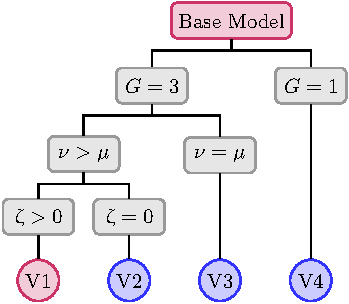
\includegraphics[width=0.4\linewidth]{variant-tree}
  \caption{Summary of four structural model variants
    with respect to simulated risk group dynamics.
    $\nu$:~rate of population entry,
    $\mu$:~rate of population exit,
    $G$:~number of risk groups,
    $\zeta$:~rates of population turnover}
  \label{fig:variant-tree}
\end{figure}
\par
In order to facilitate fair comparisons across model variants with respect to parameter values,
we start from the base model describe above above (V1),
and aim to make simplifications which have only a singular impact on the system.
For example, when moving from $\nu > \mu$ to $\nu = \mu$,
we ensure the average duration of individuals in the model $\mu^{-1}$ is unchanged
by fixing $\mu$ and reducing $\nu$ to match (V4).
Similarly, when collapsing the stratification of risk groups from $G = 3$ to $G = 1$ (V3),
we define the contact rate $C$ for all individuals as
the weighted average of previously risk-stratified $C$.
Finally, considering rates of turnover $\zeta$
(which are only applicable to V1~and~V3)
we fully determine the system, as outlined in Section~\ref{sss:params-turnover},
by specifying the average duration of individuals in each group $\bm{\delta}$,
and balancing the number of individuals moving between two groups in both directions. % TODO: add this to system section
The resulting parameter values for each scenario are summarized in Table~\ref{tab:params-variants}.
\begin{table}
  \centering
  \caption{Model parameters for structural variants.
    All rates have units $\mathrm{year}^{-1}$ and durations are in $\mathrm{years}$.}
  \label{tab:params-variants}
  \begin{threeparttable}
\begin{tabularx}{0.95\linewidth}{c *{4}{Y}}
	\toprule
	  Parameter    & Full                     & V1                           & V2                       & V3                                         \\
	\midrule
	$\bm{\hat{x}}$ & $[ 0.05\es0.20\es0.75 ]$ & ---                          & $[ 0.05\es0.20\es0.75 ]$ & $[ 0.05\es0.20\es0.75 ]$                   \\
	$\bm{\hat{e}}$ & $[ 0.05\es0.20\es0.75 ]$ & ---                          & $[ 0.05\es0.20\es0.75 ]$ & $[ 0.05\es0.20\es0.75 ]$                   \\
	     $C$       & $[ 25\es5\es1 ]$         & $[ \textbf{3} ]$\tnote{a}    & $[ 25\es5\es1 ]$         & $[ 25\es5\es1 ]$                           \\
	   $\delta$    & $[ 5\es15\es25 ]$        & $[ \textbf{33.3} ]$\tnote{b} & $[ 5\es15\es25 ]$        & $[ \textbf{33.3\es33.3\es33.3} ]$\tnote{b} \\
	    $\nu$      & $0.05$                   & $0.05$                       & $\textbf{0.03}$\tnote{c} & $0.05$                                     \\
	    $\mu$      & $0.03$                   & $0.03$                       & $0.03$                   & $0.03$                                     \\
	\bottomrule
\end{tabularx}
\footnotesize
\begin{tablenotes}
  \item
  $\bm{\hat{x}}$: proportion of individuals in the model by risk group (high, medium, low);
  $\bm{\hat{e}}$: proportion of individuals entering the model by risk group;
  $C$: rate of contact formation by risk group (per year);
  $\delta$: average duration in each risk group (years);
  $\nu$: rate of population entry (per year);
  $\mu$: rate of exit (per year).
  \item[a] Weighted average of risk-stratified $C$
  \item[b] Without turnover, duration in all groups must be equal to the inverse of the exit rate, $\mu^{-1}$
  \item[c] Adjusting the entry rate, versus exit rate, does not affect average duration in the model
\end{tablenotes}
\end{threeparttable}
\end{table}
For each model variant,
we project the simulated epidemic using these fixed parameter values,
and calculate the incidence and prevalence for each risk group, as well as overall.
Comparing the results, we highlight trends in the projected outputs
across the structural variants.
% ==================================================================================================
\subsection{Impact of Turnover}\label{ss:exp-turnover}
The overall impact of risk group turnover in an epidemic is not straightforward.
On one hand, movement of infected individuals from high to low risk groups
increases disease penetration in the lower risk groups;
however, turnover also decreases the duration of risk exposure
among individuals in the higher risk groups.
In order to clarify which effect dominates when, % JK: "dominates" -> another word?
we additionally explore a wide range of turnover magnitudes with model variant V1.
Moreover, since the average exposure experienced by each group
is directly affected by the duration of infectiousness $\delta_I$, we also explore
the impact of treatment rate $\tau = {\delta_I}^{-1}$ on this result.
\par
Since particular turnover rates $\zeta_{ij}$ are difficult to conceptualize,
we leverage the methods outlined in Section~\ref{sss:params-turnover}
to derive the necessary transition matrix given specified durations $\delta_i$
in each risk group, which are inversely correlated to turnover rates.
That is, we actually vary $\bm{\delta}$, and calculate $\zeta$ to ensure
risk group proportions $\bm{\hat{x}}$ are maintained over time.%
\footnote{Throughout this work,
  we define duration $\delta_i$ as a ``single average pass through the group''
  which does not consider reentrance after exiting to another group.}
Furthermore, we balance the absolute number of individuals
moving between two groups via turnover as in Eq.~(\ref{eq:abs-balance}),
define the duration in the medium risk group as
a linear function of $\delta_H$ like:
$\delta_M = \delta_H + 0.3\left(\mu^{-1} - \delta_H\right)$, and
the leave the duration in the high risk group as a free parameter
to allow a consistent solution.
Using this approach, a single parameter $\delta_H$ controls
the magnitude of turnover for the entire system,%
\footnote{Note that from Eq.~(\ref{eq:duration-group}), we can see that
  no risk-group duration can exceed the overall duration in the model $\mu^{-1}$.}
and so the values of $\bm{\hat{e}}$ and $\zeta$ required
to maintain group proportions $\bm{\hat{x}}$
can be resolved using Eq.~(\ref{eq:system-matrix}).
% JK: I feel like these limits need justification,
% but its difficult to give without grounding in any specific infections
To explore the impact of turnover on the model,
the duration in the high risk group $\delta_H$ is then varied from 3~to~33 years,
and the duation of infectiousness $\delta_I$ from 1~to~20 years (using the rate treatment $\tau$).
% ==================================================================================================
\subsection{Implications for Model Fitting}\label{ss:exp-turnover-fit}
Finally, since almost all context-specific applications of epidemic models entail
fitting uncertain model parameters to data-driven calibration targets,
we explore some potential implications of omitting turnover from a fitted model.
In particular, we calibrate model variants V1 (includes turnover) and V2 (no turnover) to
25\% prevalence in the high risk group, and
5\% prevalence in the low risk group,
at quasi-equilibrium, by fitting the contact rate of groups $C_H$ and $C_L$.%
\footnote{The negative log-likelihood of each predicted prevalence
  (assuming a sample size of 1000)
  was minimized using the Sequential Least SQuares Programming (SLSQP) method~\citep{Kraft1988}
  from the \texttt{scipy.optimize.minimize} Python package.}
We then compare the fitted contact rates,
and estimate the transmission population attributable fraction (TPAF)~\citep{Mishra2012}
of the high risk group,
using both the pre-calibration and post-calibration models (4 total variants).
TPAF estimates the proportion of cumulative new infections which are attributable to
prevention gaps among a specific population.
In this case, we toggle transmission ``from'' the high risk group (not ``to'').
We aim to highlight potential differences in estimation of TPAF
due to omission of turnover in models, before and after model fitting.
